% ******************************************************************	********************************************
%
% **************************************************************************************************************
\documentclass[ twoside,openright,titlepage,numbers=noenddot,%
				toc=bibliography,toc=listof,%
                footinclude=false,headinclude=false,cleardoublepage=empty,%
				BCOR=5mm,paper=a4,fontsize=11pt
                %,ngerman%
                ]{scrreprt}
%***************************************************************************************************************
% Note: Make all your adjustments in here
%***************************************************************************************************************
% ****************************************************************************************************
% htwsaar-i-mst-config.tex 
% ****************************************************************************************************  
\RequirePackage[utf8]{inputenc}				
 \DeclareUnicodeCharacter{00A0}{~}								
\RequirePackage[T1]{fontenc} 
								
% ****************************************************************************************************
% 1. Personal data and user ad-hoc commands
% ****************************************************************************************************
\newcommand{\myTitle}{Eine \LaTeX-Vorlage für Abschlussarbeiten im Bereich Informatik/Mechatronik-Sensortechnik (inkl. DFHI) an der htw saar}
\newcommand{\myDegree}{Bachelor of Science (B.\,Sc.)\xspace}
%\newcommand{\myDegree}{Master of Science (M.\,Sc.)\xspace}
\newcommand{\myDegreeType}{Bachelor\xspace}
%\newcommand{\myDegreeType}{Master\xspace}
\newcommand{\myDegreeCourse}{Praktische Informatik}
%\newcommand{\myDegreeCourse}{Informatik und Web-Engineering}
%\newcommand{\myDegreeCourse}{Kommunikationsinformatik}
%\newcommand{\myDegreeCourse}{Produktionsinformatik}
\newcommand{\myName}{Max Muster\xspace}
\newcommand{\myUni}{Hochschule für Technik und Wirtschaft des Saarlandes\xspace}
\newcommand{\myCompany}{SoftwareCenter Musterhausen\xspace}
\newcommand{\myFirstProf}{Prof. Dr.-Ing. André Miede\xspace}
\newcommand{\mySecondProf}{Prof. Dr. Thomas Kretschmer\xspace}
\newcommand{\myLocation}{Saarbrücken\xspace}
\newcommand{\myTime}{Tag.~Monat~Jahr\xspace}
\newcommand{\currentVersion}{Version 2.25, August 2024\xspace} % TODO: ggf. über git Versionsinformationen automatisch bereitstellen und verwenden

% ********************************************************************
% Setup, finetuning, and useful commands
% ********************************************************************
\newcounter{dummy} % necessary for correct hyperlinks (to index, bib, etc.)
% ****************************************************************************************************


% ****************************************************************************************************
% 2. Loading some handy packages
% ****************************************************************************************************
% ******************************************************************** 
% Packages with options that might require adjustments
% ******************************************************************** 
\PassOptionsToPackage{ngerman}{babel}   % change this to your language(s)
 \RequirePackage{babel}					
 \RequirePackage{csquotes}
	
\PassOptionsToPackage{language=auto,style=numeric-comp,backend=bibtex8,bibencoding=ascii,maxbibnames=50}{biblatex} % backend ggf. auf neueres Werkzeug (z.B. biber) anpassen
 \RequirePackage{biblatex}	
 %\bibliography{Bibliography}	% alter Befehl
 \addbibresource{Bibliography}

\PassOptionsToPackage{fleqn}{amsmath}		% math environments and more by the AMS 
 \RequirePackage{amsmath}

% ******************************************************************** 
% Setting up the page and margins
% ******************************************************************** 
\usepackage{geometry}
 \geometry{a4paper,left=25mm,right=35mm,top=25mm,bottom=30mm}
% DIESE WERTE SIND NICHT ZU VERÄNDERN -- DO NOT CHANGE THESE VALUES

% ******************************************************************** 
% General useful packages
% ******************************************************************** 
%\usepackage[automark]{scrpage2}
\PassOptionsToPackage{dvipsnames}{xcolor}
	\RequirePackage{xcolor} % [dvipsnames]  
	\definecolor{ingwi}{cmyk}{.9,0,0,0}
\usepackage{textcomp} % fix warning with missing font shapes
\usepackage{scrhack} % fix warnings when using KOMA with listings package          
\usepackage{xspace} % to get the spacing after macros right  
\usepackage{mparhack} % get marginpar right
%\usepackage{fixltx2e} % fixes some LaTeX stuff <-- ist seit 2015 nicht mehr notwendig
\PassOptionsToPackage{printonlyused}{acronym}
	\usepackage{acronym} % nice macros for handling all acronyms in the thesis
%\renewcommand{\bflabel}[1]{{#1}\hfill} % fix the list of acronyms
\usepackage{booktabs}
\usepackage{multirow}
\usepackage{todonotes} %Settings for ToDoNotes
% Eigene Shortcuts fuer laengere Befehle
	\newcommand{\todox}[1]{\todo[inline, size=\small]{#1}}
	%Nummerierte Anmerkungen
	\newcounter{todocounter}
	\renewcommand{\todox}[2][]{\stepcounter{todocounter}\todo[inline, size=\small,caption={\thetodocounter: #2}, #1]{\renewcommand{\baselinestretch}{0.5}\selectfont\thetodocounter: #2\par}}
\usepackage{blindtext}
%\usepackage{footmisc}
% ****************************************************************************************************


% ****************************************************************************************************
% 3. Setup floats: tables, (sub)figures, and captions
% ****************************************************************************************************
\usepackage{tabularx} % better tables
	\setlength{\extrarowheight}{3pt} % increase table row height
%\newcommand{\myfloatalign}{\centering} % to be used with each float for alignment
\usepackage{caption}
\captionsetup{format=hang,font=small}
\usepackage{subfig}
\usepackage{wrapfig}
% ****************************************************************************************************


% ****************************************************************************************************
% 6. Setup code listings
% ****************************************************************************************************
\usepackage{listings} 
%\lstset{emph={trueIndex,root},emphstyle=\color{BlueViolet}}%\underbar} % for special keywords
\lstset{language=[LaTeX]Tex,%C++,
    keywordstyle=\color{RoyalBlue},%\bfseries,
    basicstyle=\small\ttfamily,
    %identifierstyle=\color{NavyBlue},
    commentstyle=\color{Green}\ttfamily,
    stringstyle=\rmfamily,
    numbers=none,%left,%
    numberstyle=\scriptsize,%\tiny
    stepnumber=5,
    numbersep=8pt,
    showstringspaces=false,
    breaklines=true,
    frameround=ftff,
    frame=single,
		texcl=true,
    belowcaptionskip=.75\baselineskip
    %frame=L
} 
%Styles für verschiedene Sprachen festlegen, z.B. Java
\lstdefinestyle{Java}{
belowcaptionskip=1\baselineskip,
  breaklines=true,
  xleftmargin=\parindent,
  language=Java,
	texcl=true,
  showstringspaces=false,
  basicstyle=\footnotesize\ttfamily,
  keywordstyle=\bfseries\color{green!40!black},
  commentstyle=\itshape\color{purple!40!black},
  identifierstyle=\color{blue},
  stringstyle=\color{orange}}
% ****************************************************************************************************    		   


% ****************************************************************************************************
% 6. PDFLaTeX, hyperreferences and citation backreferences
% ****************************************************************************************************
% ********************************************************************
% Using PDFLaTeX
% ********************************************************************
\usepackage{xurl}  % better handling of long URLs / hyphenation
\PassOptionsToPackage{pdftex,hyperfootnotes=false,pdfpagelabels}{hyperref}
	\usepackage{hyperref}  % backref linktocpage pagebackref
\pdfcompresslevel=9
\pdfadjustspacing=1 
\PassOptionsToPackage{pdftex}{graphicx}
	\usepackage{graphicx} 
    

% ********************************************************************
% Hyperreferences
% ********************************************************************
\hypersetup{%
    %draft,	% = no hyperlinking at all (useful in b/w printouts)
    pdfstartpage=1, pdfstartview=Fit,%
	colorlinks=true, linktocpage=true,
	%urlcolor=Black, linkcolor=Black, citecolor=Black, %pagecolor=Black,%
	%urlcolor=brown, linkcolor=RoyalBlue, citecolor=green, %pagecolor=RoyalBlue,%
    % uncomment the following line if you want to have black links (e.g., for printing)
    colorlinks=false, pdfborder={0 0 0},
    breaklinks=true, pdfpagemode=UseNone, pageanchor=true, pdfpagemode=UseOutlines,%
    plainpages=false, bookmarksnumbered, bookmarksopen=true, bookmarksopenlevel=1,%
    hypertexnames=true, pdfhighlight=/O,%nesting=true,%frenchlinks,%
    pdftitle={\myTitle},%
    pdfauthor={\textcopyright\ \myName, \myUni},%
    pdfsubject={},%
    pdfkeywords={},%
    pdfcreator={pdfLaTeX},%
    pdfproducer={LaTeX with hyperref}%
}   

% ********************************************************************
% Setup autoreferences
% ********************************************************************
% There are some issues regarding autorefnames
% http://www.ureader.de/msg/136221647.aspx
% http://www.tex.ac.uk/cgi-bin/texfaq2html?label=latexwords
% you have to redefine the makros for the 
% language you use, e.g., american, ngerman
% (as chosen when loading babel/AtBeginDocument)
% ********************************************************************
\makeatletter
\@ifpackageloaded{babel}%
    {%
       \addto\extrasamerican{%
					\renewcommand*{\figureautorefname}{Figure}%
					\renewcommand*{\tableautorefname}{Table}%
					\renewcommand*{\partautorefname}{Part}%
					\renewcommand*{\chapterautorefname}{Chapter}%
					\renewcommand*{\sectionautorefname}{Section}%
					\renewcommand*{\subsectionautorefname}{Section}%
					\renewcommand*{\subsubsectionautorefname}{Section}% 	
				}%
       \addto\extrasngerman{% 
					\renewcommand*{\chapterautorefname}{Kapitel}%
					\renewcommand*{\sectionautorefname}{Abschnitt}%
					\renewcommand*{\subsectionautorefname}{Abschnitt}%
					\renewcommand*{\subsubsectionautorefname}{Abschnitt}% 
					\renewcommand*{\paragraphautorefname}{Absatz}%
					\renewcommand*{\subparagraphautorefname}{Absatz}%
					\renewcommand*{\footnoteautorefname}{Fußnote}%
					\renewcommand*{\FancyVerbLineautorefname}{Zeile}%
					\renewcommand*{\theoremautorefname}{Theorem}%
					\renewcommand*{\appendixautorefname}{Anhang}%
					\renewcommand*{\equationautorefname}{Gleichung}%        
					\renewcommand*{\itemautorefname}{Punkt}%
				}%	
			% Fix to getting autorefs for subfigures right (thanks to Belinda Vogt for changing the definition)
			\providecommand{\subfigureautorefname}{\figureautorefname}%  			
    }{\relax}
\makeatother


% ****************************************************************************************************
% 6. Last calls before the bar closes
% ****************************************************************************************************
% ********************************************************************
% Development Stuff
% ********************************************************************
%\listfiles
\PassOptionsToPackage{l2tabu,orthodox,abort}{nag}
	\usepackage{nag}
%\PassOptionsToPackage{warning, all}{onlyamsmath}
%	\usepackage{onlyamsmath}


% ****************************************************************************************************
% 7. Further adjustments (experimental)
% ****************************************************************************************************
%\usepackage{tocbibind} %Allows us to add Bibliography to ToC
\usepackage{enumitem}
\setdescription{font=\normalfont\bfseries} %Changes the appearance of description items
\usepackage[activate={true,nocompatibility},final,tracking=true,kerning=true,spacing=true,factor=1100,stretch=10,shrink=10]{microtype}


% ********************************************************************
% Using different fonts
% ********************************************************************
%\usepackage{lmodern} % <-- no osf support :-(
%\usepackage[tt=false]{libertine} % [osf]
%\usepackage{luximono} 
%\usepackage[urw-garamond]{mathdesign} <-- no osf support :-(
\usepackage{mathpazo} 
%\usepackage{libertinus} % math? osf?

\setkomafont{disposition}{\bfseries}
% ****************************************************************************************************

%********************************************************************
% Hyphenation
%*******************************************************
%\hyphenation{put special hyphenation here}

% ********************************************************************
% GO!GO!GO! MOVE IT!
%*******************************************************
\begin{document}
\frenchspacing
\raggedbottom
\selectlanguage{ngerman} % american ngerman
\pagenumbering{roman}
\pagestyle{plain}
%*******************************************************
% Frontmatter
%*******************************************************
%*******************************************************
% Titlepage
% [Nicht zu verändern]
%*******************************************************
\begin{titlepage}\linespread{1.5}\selectfont

\includegraphics[width=\linewidth]{Graphics/htwsaar_Logo_inwi_head_VF_4C_crop}
  \begin{center}
    \large  
    \hfill
    \vfill
    \begingroup
      \Large\bfseries Ausarbeitung 
    \endgroup
		
		\bigskip
		
    zum Thema Lambda-Architektur \\
    im Rahmen des Kurses Software-Architektur \\
    an der \myUni \\
    
  \vfill
	
  \begingroup
    \Large\bfseries\myTitle 
  \endgroup
	
	\bigskip
	
  vorgelegt von \\
  Tobias Kronser \\
  Moritz Schönenberger \\
  Leon Weyand \\
	
  \vfill
	
  betreut und begutachtet von \\
  \myFirstProf 
	
  \vfill
	
  \myLocation, \myTime                   

    \end{center}       
\end{titlepage}   
%%*******************************************************
% Titlepage
% [Nicht zu verändern]
%*******************************************************
\begin{titlepage}\linespread{1.5}\selectfont
\noindent
\includegraphics[width=3cm]{Graphics/logo-dfhi} \hfill 
\includegraphics[width=3cm]{Graphics/logo-uni-de-lorraine} \medskip

\noindent
\includegraphics[width=\linewidth]{Graphics/htwsaar_Logo_inwi_head_VF_4C_crop}

  \begin{center}
    \large  
    \hfill
    \vfill
    \begingroup
      \Large\bfseries\myDegreeType-Thesis 
    \endgroup
		
	\bigskip
		
    zur Erlangung des akademischen Grades \\
    \myDegree \\ 
    an der \myUni \\
	und \\
	der Université de Lorraine, Metz \\ 
    im Studiengang \myDegreeCourse \\
    des Deutsch-Französischen Hochschulinstituts (DFHI / ISFATES) \\ 
    
  \vfill
	
  \begingroup
    \Large\bfseries\myTitle 
  \endgroup
	
	\bigskip
	
  vorgelegt von \\
  \myName
	
  \vfill
	
  betreut und begutachtet von \\
  \myFirstProf \\
  \mySecondProf 
	
  \vfill
	
  \myLocation, \myTime                   

    \end{center}       
\end{titlepage}    % <-- für DFHI-Studiengänge
\cleardoublepage%*******************************************************
% Declaration
% [Nicht übersetzen, 
% weil Prüfungsleistung an dt. Hochschule]
%*******************************************************
\pdfbookmark[0]{Selbständigkeitserklärung}{declaration}
\chapter*{Selbständigkeitserklärung}
%\thispagestyle{empty}

Ich versichere, dass ich die vorliegende Arbeit (bei einer Gruppenarbeit: den entsprechend gekennzeichneten
Anteil der Arbeit) selbständig verfasst und keine anderen als die angegebenen Quellen und
Hilfsmittel benutzt habe.

Ich erkläre hiermit weiterhin, dass die vorgelegte Arbeit zuvor weder von mir noch von einer anderen Person an dieser oder einer
anderen Hochschule eingereicht wurde.

Darüber hinaus ist mir bekannt, dass die Unrichtigkeit dieser Erklärung eine Benotung der 
Arbeit mit der Note "`nicht ausreichend"' zur Folge hat und einen Ausschluss von der Erbringung 
weiterer Prüfungsleistungen zur Folge haben kann.
\bigskip
 
\noindent\textit{\myLocation, \myTime}

\smallskip

\begin{flushright}
    \begin{tabular}{m{5cm}}
        \\ \hline
        \centering\myName \\
    \end{tabular}
\end{flushright}
%\cleardoublepage%*******************************************************
% Sperrvermerk 
% [Nicht übersetzen, 
% weil Prüfungsleistung an dt. Hochschule]
%*******************************************************
% Der Sperrvermerk kann entfernt werden, wenn die Arbeit z.B. nicht im 
% Zusammenarbeit mit einem Unternehmen angefertigt wurde oder kein
% Sperrvermerk verlangt wird.

\pdfbookmark[0]{Sperrvermerk}{sperrvermerk}
\chapter*{Sperrvermerk}
%\thispagestyle{empty}

Die vorliegende Arbeit mit dem Titel "`\myTitle"' enthält vertrauliche Daten des Unternehmens \myCompany.

Die Arbeit darf nur dem Erst- und Zweitgutachter sowie befugten Mitgliedern des Prüfungsausschusses zugänglich gemacht werden. 
Eine Veröffentlichung und Vervielfältigung der Arbeit ist -- auch in Auszügen -- nicht gestattet.

Eine Einsichtnahme der Arbeit durch Unbefugte bedarf einer ausdrücklichen Genehmigung des Verfassers und des Unternehmens \myCompany.
 % <-- sollte in der Regel nicht notwendig sein und mit Betreuer/Unternehmen abgeklärt werden
\cleardoublepage%*******************************************************
% Abstract
%*******************************************************
\pdfbookmark[0]{Zusammenfassung}{Zusammenfassung}
\chapter*{Zusammenfassung}
Kurze Zusammenfassung des Inhaltes in deutscher Sprache, der Umfang beträgt zwischen einer halben und einer ganzen DIN A4-Seite.

Orientieren Sie sich bei der Aufteilung bzw. dem Inhalt Ihrer Zusammenfassung an Kent Becks Artikel: \url{http://plg.uwaterloo.ca/~migod/research/beckOOPSLA.html}.
\cleardoublepage%*******************************************************
% Table of Contents
%*******************************************************
\setcounter{tocdepth}{2} % <-- 2 includes up to subsections in the ToC
\setcounter{secnumdepth}{3} % <-- 3 numbers up to subsubsections

\pdfbookmark[0]{\contentsname}{toc}
\tableofcontents 

% Die weiteren Verzeichnisse folgen am Ende des Dokuments 

                  


%*******************************************************
% Mainmatter
%*******************************************************
\cleardoublepage
\pagenumbering{arabic}
\pagestyle{headings}
%\pagestyle{scrheadings}
\cleardoublepage\chapter{Einleitung}

Im Rahmen der Vorlesung \quotes{Software-Architektur} haben wir eine Fallstudie zur Lambda-Architektur durchgeführt.
In diesem Kapitel erläutern wir zunächst, warum wir uns für die Betrachtung dieser Architektur entschieden haben. 
Wir stellen die Idee unserer Fallstudie dar, in welcher ein simuliertes Parkhaussystem analysiert wird.
Anschließend definieren wir die Forschungsziele, die wir mit dieser Fallstudie erreichen wollen,
und geben einen Überblick über die eingesetzten Technologien.

\section{Motivation}
Heutzutage werden immer größere Datenmengen verarbeitet. Moderne Anwendungen müssen daher in der Lage sein, große Datenströme effizient zu verarbeiten, zu speichern und bereitzustellen, ohne dabei Verlust an Leistung oder Zuverlässigkeit zu riskieren.

Ein zentrales Problem bei der Verarbeitung großer Datenmengen wird durch das CAP-Theorem beschrieben. Dieses Theorem besagt, dass ein verteiltes Datensystem immer drei grundlegende Eigenschaften berücksichtigen muss:
\begin{itemize}
	\item \textbf{Consistency (Konsistenz)}: Jeder Lesevorgang liefert entweder den aktuellsten verfügbaren Wert oder schlägt fehl.
	\item \textbf{Availability (Verfügbarkeit)}: Jede Anfrage erhält garantiert eine Antwort, auch wenn einige Knoten des Systems ausgefallen sind.
	\item \textbf{Partition Tolerance (Partitionstoleranz)}: Das System funktioniert weiter, auch wenn Teile des Netzes ausfallen oder Kommunikationsprobleme auftreten.
\end{itemize}

Allerdings definiert das CAP-Theorem hierbei eine grundlegende Einschränkung:
Ein System kann immer nur zwei dieser drei Eigenschaften garantieren. 
In datenintensiven Anwendungen, die eine hohe Fehlertoleranz (Partition Tolerance) und Verfügbarkeit (Availability) erfordern, kann daher nicht sichergestellt werden, dass jede Abfrage immer die aktuellsten Daten liefert. Dies stellt eine große Herausforderung für Systeme dar, die sowohl Echtzeitdatenverarbeitung als auch Langzeitanalysen ermöglichen sollen.

Die Lambda-Architektur ist ein Architekturmuster, das speziell für Big-Data-Anwendungen entwickelt wurde, also für Systeme, die große Datenmengen effizient verarbeiten müssen. Ihr Ziel ist es, eine fehlertolerante und hochverfügbare Architektur bereitzustellen, die trotz der Einschränkungen des CAP-Theorems eine möglichst hohe Datenkonsistenz gewährleistet. Sie begegnet dem Problem des CAP-Theorems, indem sie zwei Verarbeitungswege kombiniert: den Batch Layer für konsistente Langzeitanalysen und den Speed Layer für schnelle Echtzeitabfragen.

In dieser Fallstudie wollen wir diese Eigenschaften der Lambda-Architektur analysieren und bewerten. Dazu simulieren wir einen realen Anwendungsfall, in dem sowohl die Langzeitanalyse großer Datenmengen als auch die schnelle Bereitstellung neuer Daten eine zentrale Rolle spielen.

Wir orientieren uns dabei an bestehenden Anwendungsgebieten der Lambda-Architektur. Diese Architektur ist insbesondere in Web- und IoT-Anwendungen weit verbreitet, da sie eine skalierbare Verarbeitung großer Datenmengen bei gleichzeitig schneller Verfügbarkeit aktueller Daten ermöglicht.

\todo[inline]{Parkhaus = IoT-Anwendung? SmartCity? Anderes?}
Für unsere konkrete Fallstudie haben wir uns für eine IoT-Anwendung im Bereich der Parkhausanalyse entschieden.
Ziel ist es, ein Parkhaussystem zu simulieren, das mithilfe von Kameras die Ein- und Ausfahrten in mehreren Parkhäusern erfasst und analysiert.
\todo[inline]{fahrzeugspezifische Informationen (Breite etc?) in serving layer überhaupt verfügbar? wenn nicht, trotzdem erwähnen?}
Dabei sollen fahrzeugspezifische Informationen gespeichert und verarbeitet werden. 
Dieses Szenario eignet sich aus unserer Sicht gut für die Lambda-Architektur, da sich Anwendungsfälle sowohl für Langzeitanalysen (z.B. Belegungsmuster über mehrere Wochen) als auch für Echtzeitabfragen (z.B. aktuelle Parkplatzverfügbarkeit) ergeben.


\section{Forschungsfragen}
Mit dem Ziel unserer Fallstudie vor Augen können wir die folgenden Forschungsfragen definieren, die wir durch unsere Implementierung der Lambda-Architektur beantworten möchten:
\begin{itemize}
	\item \textbf{RQ1:} Mit welchen Technologien kann eine Lambda-Architektur umgesetzt werden?
	\item \textbf{RQ2:} Welche architektonischen Eigenschaften der Lambda-Architektur lassen sich in unserer Fallstudie identifizieren?
	\item \textbf{RQ3:} Was sind Vor- und Nachteile der Lambda-Architektur?
	\item \textbf{RQ4:} Welche Herausforderungen treten bei der Implementierung der Lambda-Architektur in einer kleinen, nicht skalierten Umgebung auf?
\end{itemize}

\section{Forschungsansatz}
Unser Ziel in dieser Fallstudie ist es, eine einfache, aber funktionsfähige Implementierung der Lambda-Architektur in einer simulierten Umgebung zu entwickeln. Der Fokus liegt dabei nicht auf der Entwicklung einer produktionsreifen Lösung für ein reales Parkhaussystem, sondern vielmehr auf der Schaffung eines praxisnahen Szenarios, das hilft, die Architektur besser zu verstehen und ihre Vor- und Nachteile zu evaluieren.

Um dieses Ziel zu erreichen, entwickeln wir eine Datenquelle, die Ein- und Ausfahrten verschiedenartiger Autos simuliert.
Diese Daten durchlaufen die verschiedenen Schichten der Lambda-Architektur, so dass sowohl Echtzeit- als auch Batch-Verarbeitung getestet werden können.

Um die erste Forschungsfrage (RQ1) zu beantworten, haben wir uns für bewährte Open-Source-Technologien entschieden.
Anstatt eine eigene Architektur von Grund auf neu zu entwickeln, verwenden wir existierende Werkzeuge, die bereits in der Praxis für die Lambda-Architektur eingesetzt werden. Die Auswahl basiert auf einer Literaturrecherche zu typischen Technologien für die drei Schichten der Lambda-Architektur. Eine detaillierte Erläuterung der Komponenten und Funktionsweisen der Lambda-Architektur erfolgt in Kapitel 2.

Der Speed Layer der Lambda-Architektur ist für die Echtzeitverarbeitung zuständig. Im Speed Layer müssen die Daten schnell verarbeitet werden. Für die Implementierung des Speed Layers wurde daher Apache Kafka gewählt. Kafka ermöglicht eine schnelle und zuverlässige Verarbeitung und Weiterleitung von Datenströmen.

Der Serving Layer übernimmt die Aggregation und Bereitstellung der verarbeiteten Daten. Er verbindet den Speed- und den Batch-Layer und bietet eine zusammenführende Sicht auf die gespeicherten Informationen. Wir haben uns entschieden, den Serving Layer mit Apache Cassandra zu realisieren. Cassandra ist eine NoSQL-Datenbank, die speziell für schnelle Abfragen optimiert ist und in vielen realen Implementierungen der Lambda-Architektur für den Serving Layer verwendet wird.

Im Batch Layer werden alle historischen Rohdaten gespeichert und verarbeitet. In der klassischen Lambda-Architektur werden hier häufig verteilte Systeme wie Apache Hadoop oder Apache Spark eingesetzt, da diese für den Umgang mit großen Datenmengen optimiert sind. Da in unserer Fallstudie jedoch nicht mit so großen Datenmengen gearbeitet wird, verzichten wir auf eine skalierbare, verteilte Speicherung. Stattdessen verwenden wir auch hier Apache Cassandra, da es sowohl für schnelle Lesezugriffe als auch für die Langzeitspeicherung großer Datenmengen optimiert ist. 

Die Anwendung wird in C\# entwickelt, da diese Sprache eine gute Integration mit Apache Kafka und Apache Cassandra bietet. Für die Verwaltung und Bereitstellung der verschiedenen Komponenten verwenden wir Docker. Diese Container-Technologie ermöglicht eine einfache Installation, Verwaltung und Reproduzierbarkeit unserer Umgebung, da alle benötigten Dienste in isolierten Containern laufen und unabhängig von der Konfiguration des Host-Systems sind.
	 	% Diese Einbindungen werden natürlich entfernt, wenn es an die richtige
\cleardoublepage\chapter{Verwandte Arbeiten}
% \todo[inline]{Kapitelname ueberdenken (hab angst vor umlauten in umgebungen), hier auch beschreibung was lambda ueberhaupt ist}
In diesem Kapitel geben wir einen Überblick über bestehende Arbeiten zur Lambda-Architektur und deren Einfluss auf die Entscheidungen, die wir bei der Entwicklung unserer Fallstudie getroffen haben. Zunächst erläutern wir die grundlegende Struktur der Lambda-Architektur, ihre Kernkomponenten und ihre Ziele. Anschließend betrachten wir existierende Implementierungen, die als Inspiration für unser eigenes Fallstudienszenario dienten.

Darauf aufbauend analysieren wir die architektonischen Eigenschaften der Lambda-Architektur sowie ihre bekannten Vor- und Nachteile, um eine Grundlage für die spätere Bewertung unserer Fallstudie zu schaffen. Abschließend vergleichen wir die Lambda-Architektur mit der Kappa-Architektur, einer alternativen Architektur, die in bestimmten Szenarien die Schwächen der Lambda-Architektur umgehen soll.

\section{Überblick über die Lambda-Architektur}
Die Lambda-Architektur wurde von Nathan Marz \cite{warren2015big} als Antwort auf die wachsenden Herausforderungen bei der Verarbeitung großer Datenmengen im Zeitalter von Big Data entwickelt. Sie entstand aus der Erkenntnis, dass herkömmliche Architekturen oft zu komplex, fehleranfällig und schwer skalierbar sind. In vielen Systemen kann bereits ein einziger Datenfehler oder der Ausfall einer Komponente dazu führen, dass das gesamte System inkonsistent wird, Daten verloren gehen oder verfälscht werden und das System nicht mehr zuverlässig arbeitet.

Ein weiteres Problem klassischer Architekturen ist, dass sie Echtzeit- und historische Daten nicht effizient kombinieren können.
Bei Big-Data-Anwendungen muss das System nicht nur jederzeit auf die Daten zugreifen und auf Anfragen reagieren können, sondern auch sicherstellen, dass die gelieferten Informationen stets aktuell sind. Dies würde bedeuten, dass bei jeder einzelnen Anfrage alle gespeicherten Daten vollständig durchsucht und verarbeitet werden müssten, um die aktuellsten Werte zu gewährleisten. Bei wachsenden Datenmengen wird dies jedoch schnell ineffizient und führt zu hohen Latenzzeiten und Systembelastungen.

Um diese Probleme zu lösen, verfolgt die Lambda-Architektur einen Ansatz, der große Datenmengen effizient verarbeitet und gleichzeitig Fehlertoleranz, Skalierbarkeit und Konsistenz gewährleistet.
Hierzu werden Berechnungen nach ihrer Komplexität in Echtzeit- und Batch-Berechnungen unterschieden.
Echtzeit-Berechnungen werden direkt auf eintreffenden Daten ausgeführt und ermöglichen eine aktuellen Überblick.
Hierzu dürfen diese nur wenig Zeit in Anspruch nehmen, weshalb es sich in der Regel um inkrementelle Berechnungen handelt.
Batch-Berechnungen werden periodisch auf der Gesamtheit aller Daten ausgeführt und können eine lange Zeit in Anspruch nehmen.
Diese Berechnungen können beliebig komplex sein, ihre Ergebnisse sind allerdings stets erst verzögert verfügbar.

Das Hauptziel der Lambda-Architektur ist es, 
die aktuellen Daten aus Echtzeit-Berechnungen mit den Ergebnissen der letzten Batch-Berechnungen zu kombinieren,
um Anfragen über historische und aktuelle Daten hinweg zu ermöglichen.
% Hierzu ist eine sorgfältige Einteilung von Berechnungen in Echtzeit-Berechnungen bzw. Batch-Berechnungen notwendig.
Hieraus ergibt sich eine Aufteilung der Architektur in drei Schichten unterteilt (siehe Abbildung 1):

\begin{itemize}
	\item \textbf{Batch Layer:} Speichert alle Rohdaten unverändert und dient als Langzeitarchiv. Dadurch können die Daten wiederholt verarbeitet und für regelmäßige Langzeitanalysen verwendet werden.
	\item \textbf{Speed Layer:} Verarbeitet Datenströme in Echtzeit, um sofortige Ergebnisse zu liefern. Da der Batch-Layer nicht für schnelle Abfragen geeignet ist, übernimmt der Speed-Layer die Aufgabe, aktuelle Daten schnell zur Verfügung zu stellen.
	\item \textbf{Serving Layer:} Verbindet Batch- und Speed-Layer und stellt die Daten für Benutzeranfragen bereit. Kombiniert die Ergebnisse der beiden Schichten und ermöglicht so eine konsistente und effiziente Datenbereitstellung.
\end{itemize}


\begin{figure}[h]
    \centering
    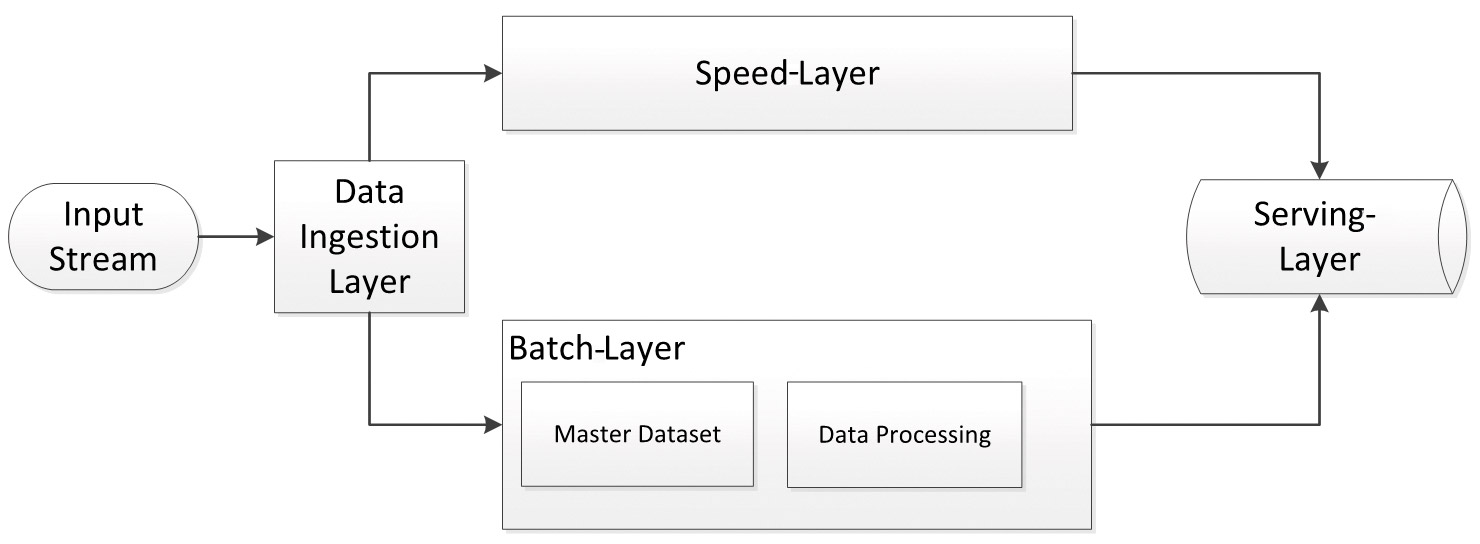
\includegraphics[width=0.8\textwidth]{Graphics/Lambda_Architecture.png}
    \caption{Aufbau der Lambda-Architektur \cite{entwickler_lambda_kappa}.}
    \label{fig:beispielbild}
\end{figure}

Durch diese klare Trennung der Verarbeitungsebenen ermöglicht die Lambda-Architektur ein Gleichgewicht zwischen geringer Latenz und hoher Genauigkeit. Während die Batch Layer eine robuste und fehlertolerante Verarbeitung großer Datenmengen gewährleistet, wäre es zu zeitaufwändig, diese Schicht bei jeder Anfrage vollständig zu durchlaufen, um aktuelle Daten bereitzustellen. Hier kommt der Speed Layer ins Spiel: Er verarbeitet neue Daten in Echtzeit und stellt sie sofort zur Verfügung, um eine schnelle Reaktionszeit zu gewährleisten.

\section{Anwendungsfälle der Lambda-Architektur}
Da traditionelle Systeme wie relationale Datenbanken und klassische Batch-Processing-Systeme zunehmend an ihre Grenzen stoßen, wenn es darum geht, die stetig wachsenden Datenmengen effizient zu verarbeiten, gewinnen Big-Data-Architekturen für moderne Anwendungen immer mehr an Bedeutung. Insbesondere im Zeitalter des Internets, in dem kontinuierlich riesige Datenmengen generiert, übertragen und analysiert werden, hat sich die Lambda-Architektur als leistungsfähige Lösung etabliert \cite{kumar2020lambda,kiran2015lambda,katkar2015study}.

Yuvraj Kumar \cite{kumar2020lambda} beschreibt in seinem Paper eine Vielzahl von modernen Anwendungsfällen der Lambda-Architektur sowie die Technologien, die häufig für deren Implementierung verwendet werden. Große Technologieunternehmen wie Twitter, LinkedIn, Netflix und Amazon nutzen die Lambda-Architektur, um ihre enormen Datenmengen effizient zu analysieren. Vor allem im Bereich der personalisierten Werbung spielt sie eine zentrale Rolle: Historische Kundendaten werden mit aktuellen Nutzerinteraktionen kombiniert, um in Echtzeit maßgeschneiderte Werbung auszuspielen.
Auch im Finanzsektor nutzen Unternehmen die Lambda-Architektur, um historische Transaktionsdaten mit Echtzeitanalysen zu verknüpfen. So können verdächtige Muster identifiziert und Betrugsversuche frühzeitig erkannt werden. Auch im Internet of Things (IoT) findet die Lambda-Architektur breite Anwendung. So wird sie beispielsweise in Smart Cities eingesetzt, um Logistikprozesse zu optimieren oder die Abfallentsorgung effizienter zu gestalten.

Das Paper von Kiran et al. \cite{kiran2015lambda} zeigt, dass insbesondere Smart City Anwendungen stark von der Lambda-Architektur profitieren, da hier große Mengen an Sensordaten kontinuierlich erfasst und analysiert werden müssen. Die Autoren beschreiben eine konkrete Implementierung der Lambda-Architektur zur Verarbeitung und Analyse von Sensordaten in einer Netzwerkumgebung. Hierzu untersuchen Kiran et al. die Verarbeitung von Netzwerk- und Sensordaten aus dem Energy Sciences Network (ESnet). Ziel der Implementierung ist die Erkennung von Anomalien und die Optimierung der Netzwerkauslastung. Die Lamda-Architektur ist für diese Anwendung besonders geeignet, da sie die gleichzeitige Verarbeitung historischer und aktueller Netzdaten ermöglicht. Während im Batch-Layer Langzeitanalysen durchgeführt werden, um wiederkehrende Muster zu identifizieren, kann der Speed-Layer Anomalien in Echtzeit erkennen und darauf reagieren. 

Die in der Literatur beschriebenen Anwendungsfälle, insbesondere die Arbeiten von Kiran et al. \cite{kiran2015lambda} und Kumar \cite{kumar2020lambda}, haben uns geholfen, ein geeignetes Szenario für unsere Fallstudie zu identifizieren. Die Forschung zeigt, dass die Lambda-Architektur besonders häufig in Smart City-Anwendungen eingesetzt wird, da sie die Echtzeitverarbeitung großer Sensordatenströme mit Langzeitanalysen kombiniert.

Darauf aufbauend wollten wir für unsere Fallstudie eine Anwendung im Smart City Kontext wählen, die ebenfalls Echtzeitanalysen mit Langzeitprognosen kombiniert. Dies führte uns schließlich zur Parkhausanalyse. Ähnlich wie in der Arbeit von Kiran et al. \cite{kiran2015lambda} ist es in unserem Szenario sinnvoll, historische Daten zur Vorhersage der Parkhausauslastung mit Echtzeitinformationen über die aktuelle Belegung zu verknüpfen.

\section{Technologien der Lambda-Architektur}
Der vorherige Abschnitt hat gezeigt, dass die Lambda-Architektur eine weit verbreitete Big-Data-Architektur ist, die bereits in einer Vielzahl von Anwendungen implementiert wurde. In der Literatur werden verschiedene Technologien beschrieben, die zur Implementierung der drei Schichten der Lambda-Architektur verwendet werden können.

Ein konkretes Beispiel für die technologische Umsetzung liefert das Paper von Kiran et al. \cite{kiran2015lambda}, das eine Cloud-basierte Implementierung der Lambda-Architektur für die Sensordatenverarbeitung beschreibt. Die Autoren verwenden unterschiedliche Technologien für den Batch Layer, den Speed Layer und den Serving Layer.

Für den Batch Layer verwenden Kiran et al. \cite{kiran2015lambda} das Apache Hadoop Distributed File System (HDFS). HDFS ist eine der am häufigsten verwendeten Technologien für die Lambda-Architektur, da es ein skalierbares, fehlertolerantes und verteiltes Dateisystem darstellt, das speziell für die Speicherung großer Datenmengen entwickelt wurde \cite{ganelin2016spark}.
Aufgrund seiner Architektur ist HDFS jedoch relativ langsam bei Lese- und Schreibzugriffen, weshalb es hauptsächlich für Batch-Processing-Aufgaben verwendet wird. In der Implementierung von Kiran et al. wird HDFS verwendet, um historische Rohsensordaten von Netzwerkroutern unverändert zu archivieren. Da Lesezugriffe auf HDFS relativ langsam sind, können periodische Batch-Analysen sehr zeitaufwändig sein.

Für die Speed Layer verwenden Kiran et al. \cite{kiran2015lambda} Apache Spark Streaming. Apache Spark ist eine vielseitige Technologie, die sowohl für Batch Processing als auch für Stream Processing eingesetzt werden kann. Spark Streaming ist eine Erweiterung von Apache Spark und ermöglicht die Verarbeitung von Datenströmen in Echtzeit, indem eingehende Daten kontinuierlich analysiert und aggregiert werden.
Der Vorteil von Spark Streaming gegenüber klassischen Batch-Technologien ist, dass es Echtzeitdatenverarbeitung mit geringer Latenz ermöglicht, ohne dass die Daten vorher vollständig gespeichert werden müssen.

Für den Serving Layer verwenden Kiran et al. \cite{kiran2015lambda} Amazon S3, um die Sensordaten aus dem Batch Layer zu aggregieren und für historische und Echtzeit-Abfragen bereitzustellen. Die Wahl von Amazon S3 basiert darauf, dass die Autoren eine Cloud-basierte Implementierung der Lambda-Architektur entwickelt haben, die auf skalierbare Speicherdienste angewiesen ist.

Im Gegensatz dazu planen wir in unserer Fallstudie eine lokale Implementierung der Lambda-Architektur, weshalb alternative Technologien für die Speicherung und Aggregation im Serving Layer in Betracht gezogen werden müssen.

In der Literatur werden zahlreiche weitere Technologien beschrieben, die für die verschiedenen Schichten der Lambda-Architektur eingesetzt werden können. Besonders hervorzuheben ist die Arbeit von Kumar \cite{kumar2020lambda}, der mehrere alternative Technologien diskutiert, die auch für unsere Fallstudie vielversprechend sind.

Laut Kumar \cite{kumar2020lambda} ist Apache Kafka eine der am häufigsten verwendeten Technologien für die Lambda-Architektur. Kafka ist ein verteiltes Publish-Subscribe-Messaging-System, das für Echtzeit-Datenströme optimiert ist \cite{kreps2011kafka}. Es ermöglicht das Publizieren neuer Daten in Echtzeit in eine Queue. Von dort aus können die Daten sowohl an den Batch-Layer zur langfristigen Speicherung als auch an den Speed-Layer zur sofortigen Verarbeitung weitergeleitet werden. Damit ist sichergestellt, dass Echtzeit- und Langzeitverarbeitung parallel erfolgen können.

Eine weitere Technologie, die laut Kumar \cite{kumar2020lambda} häufig in der Lambda-Architektur eingesetzt wird, ist Apache Cassandra. Cassandra ist eine hochskalierbare NoSQL-Datenbank, die sich besonders für den Serving Layer eignet \cite{warren2015big}. Im Serving Layer werden Echtzeitabfragen aus dem Speed Layer und aggregierte Batch Views aus dem Batch Layer zusammengeführt und gespeichert. Cassandra zeichnet sich durch schnelle Lese- und Schreibzugriffe aus, was für die kontinuierliche Aktualisierung der Daten im Serving Layer wichtig ist.

\section{Eigenschaften der Lambda-Architektur}
Nachdem wir uns in den vorherigen Abschnitten mit verschiedenen Anwendungsfällen und Technologien der Lambda-Architektur beschäftigt haben, wollen wir nun die zentralen Eigenschaften dieser Architektur näher analysieren. Basierend auf den betrachteten Anwendungsfällen identifizieren wir die wesentlichen Stärken und Schwächen der Lambda-Architektur. Diese identifizierten Eigenschaften wollen wir später als Richtlinien für die Implementierung und Evaluierung unserer Fallstudie nutzen.

\subsection{Vorteile der Lambda-Architektur}
Die Lambda-Architektur zeichnet sich durch eine klare Trennung der Datenverarbeitung in drei Schichten aus. Diese Struktur ermöglicht es, jede Schicht unabhängig voneinander zu optimieren und weiterzuentwickeln. Wie Marz \cite{warren2015big} beschreibt, sind die einzelnen Verarbeitungsebenen nur gering voneinander abhängig, so dass sie mit unterschiedlichen Technologien realisiert werden können. Dadurch kann jede Schicht flexibel ausgetauscht oder skaliert werden, ohne dass die gesamte Architektur überarbeitet werden muss. Diese Skalierbarkeit macht die Lambda-Architektur besonders geeignet für Big-Data-Anwendungen, da sie flexibel an steigende Datenmengen angepasst werden kann.

Ein weiteres zentrales Merkmal der Lambda-Architektur ist die Fehlertoleranz durch die Verwendung von Immutable Data \cite{warren2015big}. Da die Rohdaten unverändert in der Batch Layer gespeichert werden, bleiben sie jederzeit abrufbar und können erneut verarbeitet werden, ohne dass das System inkonsistent wird. Marz \cite{warren2015big} betont, dass dieser Ansatz Datenverluste nahezu ausschließt, da Daten nicht gelöscht oder überschrieben, sondern nur ergänzt werden. Tritt ein Fehler in der Verarbeitung oder in den Daten selbst auf, kann dieser durch eine erneute Verarbeitung der unveränderten Rohdaten behoben werden. Dies ist insbesondere in Anwendungen mit hohen Anforderungen an die Datenintegrität von Vorteil. Die Arbeit von Kiran et al. \cite{kiran2015lambda} zur Netzwerkanalyse im ESnet zeigt, dass diese Eigenschaft es ermöglicht, Sensordaten langfristig zu speichern und Fehler in der Netzwerkanalyse durch Nachberechnungen zu korrigieren.

\subsection{Nachteile der Lambda-Architektur}
Obwohl die Lambda-Architektur viele Vorteile bietet, bringt sie auch Nachteile mit sich. 

Die Trennung der Verarbeitungsebenen führt zu einem erhöhten Entwicklungs- und Wartungsaufwand. 
Die von Marz \cite{warren2015big} beschriebene geringe Abhängigkeit zwischen den Schichten bietet zwar Flexibilität, 
allerdings ergibt sich auch ein geringes Potenzial für gemeinsame Implementierungen beziehungsweise die Wiederverwendung von Komponenten.
Dies trifft umso mehr zu, wenn die Schichten unterschiedliche Technologien einsetzen.

Kumar \cite{kumar2020lambda} beschreibt insbesondere die hohe Komplexität der Kombination von Speed Layer und Batch Layer im Serving Layer. Da für beide Verarbeitungsebenen separate Pipelines entwickelt werden müssen, ist es notwendig, die Ergebnisse beider Ebenen in der Serving Layer zu integrieren. Diese Integration kann fehleranfällig sein und erfordert eine sorgfältige Synchronisation der Daten, um konsistente Abfragen zu gewährleisten. Während die Lambda-Architektur auf konzeptioneller Ebene einfach zu verstehen ist, stellt die technische Umsetzung eine Herausforderung dar. Die verschiedenen Schichten werden mit unterschiedlichen Open-Source-Technologien realisiert, die miteinander kommunizieren müssen \cite{katkar2015study}.

Ein weiteres Problem der Lambda-Architektur ist der hohe Speicherbedarf durch die doppelte Datenhaltung. Da sowohl die Speed Layer als auch die Batch Layer Daten speichern, werden viele Daten redundant gespeichert, um eine konsistente Verarbeitung in beiden Schichten zu gewährleisten. Während der Batch-Layer alle Rohdaten langfristig speichert, verwendet der Speed-Layer einen separaten Speicher für die Echtzeitverarbeitung. Dies führt insbesondere bei Anwendungen mit großen Datenmengen zu einem erhöhten Speicherbedarf \cite{kumar2020lambda}.
\cleardoublepage\chapter{Konzept}
\cleardoublepage\chapter{Implementierung}

Das Projekt ist in der Programmiersprache CSharp geschrieben.
Lokale Instanzen von Apache Kafka und Cassandra werden in Docker-Containern gestartet.
%TODO: Implementierung-Überblick


\section{Datenbankstruktur}

\begin{figure}[h!]%
    \centering%
    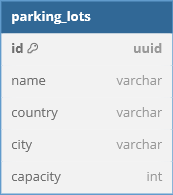
\includegraphics[width=0.3\textwidth]{Graphics/ParkingLotTable.png}%
    \caption{Parkhaus-Tabelle}%
    \label{fig:table_parking_lots}
\end{figure}%

In der Tabelle \ref{fig:table_parking_lots} sind alle Parkhäuser, die im System existieren mit ihrem Standort, sowie ihrer Kapazität, hinterlegt.
Die Daten hierin werden aktuell manuell angelegt.

\begin{figure}[h!]%
    \centering%
    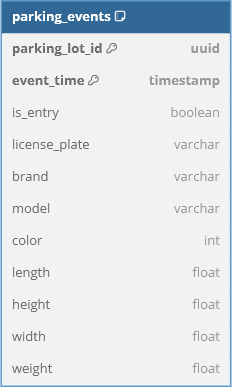
\includegraphics[width=0.3\textwidth]{Graphics/parking_events.png}%
    \caption{Parkevent-Tabelle}%
    \label{fig:table_parking_events}
\end{figure}%

In der Tabelle \ref{fig:table_parking_events} sind alle in der Vergangenheit geschehenen Park-Events gespeichert.
Jedes dieser Events stellt die Ein- beziehungsweise Ausfahrt eines Autos in ein Parkhaus dar.
Bei diesen Daten handelt es sich um reine Rohdaten, die den unverarbeiteten Daten von Parkhäusern entsprechen.

\begin{figure}[h!]%
    \centering%
    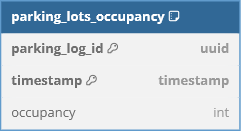
\includegraphics[width=0.3\textwidth]{Graphics/occupancy.png}%
    \caption{Zwischensummen-Tabelle}%
    \label{fig:table_occupancy}
\end{figure}%

In der Tabelle \ref{fig:table_occupancy} werden Füllstände der Parkhäuser zu bestimmten Zeitpunkten gespeichert.
In der aktuellen Konfiguration wird je Parkhaus der Füllstand zu jeweils vollen 10 Minuten berechnet.
Diese Daten werden periodisch vom Batch-Layer berechnet und können bei Bedarf, beispielsweise nach Rohdaten-Korrektur oder Batch-Prozess-Korrektur nochmal über alle Daten hinweg neu berechnet werden.

\section{Core-Bibliothek}
Auf der Core-Bibliothek bauen alle anderen Projekte auf.
In dieser Bibliothek befinden sich alle geteilten Programmteile:
\begin{itemize}
    \item \textbf{Konfiguration}: string Konstanten für Kafka-Topics, sowie Cassandra-Aufbau bestehend aus Tabellen und -Spaltennamen
    \item \textbf{Geteilte Interfaces}: ICarModel (allgemeine Autoinformationen), ICarData (ICarModel + spezifische Autoinformationen), IParkingEventData (ICarData + Parkhaus + Einfahrts- oder Ausfahrtszeit)
    \item \textbf{Geteilte Datenstrukturen}: CarEntryData (rerpäsentiert ein vollständiges Einfahrts-Event), CarExitData (rerpäsentiert ein vollständiges Ausfahrts-Event), OccupancyState (repräsentiert den exakten Füllstand eines Parkhauses zu einem gegebenen Zeitpunkt)
    \item \textbf{Serialisierungs- und Deserialisierungsfuntionen}: Datenstrukturen binär oder als String serialisieren und wiedererstellen
    \item \textbf{CassandraHelper}: Hilfsklasse, die die Verbindung zur Cassandra-Datenbank verwaltet und alle in anderen Projekten verwendeten Datenbankzugriffe mit Hilfe von CQL (Cassandra Query Language) umsetzt
    \item \textbf{Setup-Validierung}: ermöglicht Anwendungen, die Kafka oder Cassandra benötigen zu überprüfen, ob Kafka und Cassandra korrekt aufgesetzt sind
\end{itemize}


\section{Datengrundlage}
Da keine realen Daten zur Verfügung stehen, verwenden wir einen selbst geschriebenen Datengenerator, der Ein- und Ausfahrten in ein Parkhaus über Zeit simuliert.
Dabei werden Parkevent-Daten \quotes{CarEntryData} und \quotes{CarExitData} bestehend aus Parkhaus-Id, Zeitstempel, Nummernschild, Automarke, Automodell, Farbe, gemessener Länge, gemessener Breite, gemessener Höhe und gemessenem Gewicht generiert.
Die Parkevent-Daten werden dann direkt in die Kafka-Topic \quotes{car-events} geschrieben.
Ausfahrts-Events werden stets basierend auf einem zuvor generierten Einfahrts-Event, zu dem es noch kein zugehöriges Ausfahrts-Event gibt generiert.
Dieser Prozess geschieht stark beschleunigt, um einfaches Testen zu ermöglichen: Innerhalb von Minuten werden Daten für einen ganzen Tag generiert.
Um die Daten für mehrere Parkhäuser auf einmal zu generieren, können beliebig viele Parkhäuser konfiguriert werden.
Für jedes Parkhaus wird dann ein entsprechender Generator-Thread gestartet.
Der Generator berücksichtigt die maximale Kapazität eines Parkhaus und generiert morgens mehr Einfahrts-Events und abends mehr Ausfahrts-Events.
%Todo: Tabelle angeben
In der Datenbank stehen Einfahrts- und Ausfahrts-Events in der selben Tabelle und werden nur durch ein bool-Flag, bei dem \textbf{True} ein Einfahrts-Event markiert, unterschieden.


\section{Speed Layer}
Der Speed Layer beinhaltet nur ein einzelnes Projekt \quotes{SpeedLayerParkingDeckWorker}, das gleichzeitig Kafka-Consumer und Kafka-Producer ist.
Dabei handelt es sich um eine Kommandozeilenanwendung, die die eingehenden Grunddaten aus der Kafka-Topic \quotes{car-events} erhält und für ein einzelnes Parkhaus mehrere Events zu einer Zwischensumme zusammenfasst.
Diese Zwischensumme entspricht der Differenz der im Parkhaus stehenden Autos im Vergleich zum Stand vor den Events.
Wird eine Obergrenze an Park-Events für ein Parkhaus erreicht, oder ist eine Zeitspanne seit dem ersten Park-Event abgelaufen, so wird die Differenz gemeinsam mit der Parkhaus-Id in eine zweite Kafka-Topic \quotes{car-events-preprocessed} geschrieben.
Die Obergrenze an Parkevents, sowie die Zeitspanne sind im Worker konfigurierbar.
Es können beliebig viele Speed-Layer-Worker gleichzeitig gestartet werden, wobei je Parkhaus ein Speed-Layer-Worker vorgesehen ist.
Standardmäßig wird beim Starten des Projekts auch ein Worker je Parkhaus gestartet.
Durch die Verwendung der selben GruppenId (abhängig vom Parkhaus des Workers) ist es auch möglich, mehrere Worker für das selbe Parkhaus zu starten, während Kafka jedes Event nur an einen dieser Worker verteilt.
Praktisch ist das in unserer Fallstudie allerdings nicht sinnvoll, da ein einzelnes reales Parkhaus nur eine überschaubare Menge an Events produzieren kann.


\section{Batch Layer}
%TODO: Projektnamen in Repo anpassen
Das Batch Layer besteht aus mehreren Projekten:
\begin{itemize}
    \item \textbf{Kafka-Consumer} persistiert alle Grunddaten aus Kafka in der Datenbank.
    \item \textbf{Batch-Processing} führt regelmäßig verschiedene Batch-Berechnungen basierend auf den in der Datenbank persistierten Daten aus und schreibt die Ergebnisse in die Datenbank zurück. 
\end{itemize}

\subsection{KafkaConsumer}
Der Kafka-Consumer des Batch Layers ist eine Kommandozeilenanwendung, die beim Start die Kafka-Topic \quotes{car-events} abonniert und alle hier anfallenden Events erhält.
Diese Events werden dann in Cassandra übertragen, hierdurch bleiben alle Rohdaten langfristig verfügbar.
Die Übertragung geschieht der Einfachheit halber in einzelnen Datenbankoperationen.
In einem realen System, in dem mehr Daten anfallen, wäre es hingegen wichtig, die Events zu bündeln und eine Menge Events gesammelt an die Datenbank zu übertragen.
Es können beliebig viele Kafka-Consumer gleichzeitig gestartet werden.
Alle Instanzen teilen die selbe Kafka-GroupId, wodurch jedes Event nur an genau eine Instanz übertragen wird.
In der Kommandozeile werden Ein- und Ausfahrten ausgegeben.

\subsection{Batch-Processing}
Das Batch-Processing des Batch Layers ist eine Kommandozeilenanwendung, die periodisch die Daten der vergangenen halben Stunde aus der Datenbank läd und darauf basierend Füllstände je Parkhaus in 10 Minuten Intervallen berechnet.
Da der Datengenerator beschleunigt Daten generiert, läuft diese Anwendung auch beschleunigt und berechnet alle 2 Minuten die Daten einer halben Stunde.
Immer, wenn ein Batch-Vorgang abgeschlossen ist, schreibt die Anwendung eine Benachrichtigung in die Kafka-Topic \quotes{batch-notification}.
Diese Nachricht dient dem Serving Layer zu


\section{Serving Layer}
Das Serving Layer besteht nur aus einem Projekt \quotes{ServingLayer}.
Hier handelt es sich um eine Kommandozeilenanwendung, die Daten aus Kafka und Cassandra zusammenführt und für Benutzeranwendungen bereitstellt.
Beim Start liest der Serving Layer alle existierenden Parkhäuser aus der Cassandra-Datenbank und legt sich je Parkhaus einen Cache an.
Dazu werden die Kafka-Topics \quotes{car-events-preprocessed}, deren Daten im Speed Layer berechnet werden, und \quotes{batch-notification} abonniert.
Dieser Cache beinhaltet die aktuelle Anzahl an Autos im Parkhaus, die sich aus dem Ergebnis des letzten Batch-Views, sowie der seitdem angefallenen Summe an Park-Events in \quotes{car-events-preprocessed} ergibt.
Immer wenn eine Nachricht in \quotes{batch-notification} den Abschluss eines weiteren Batch-Vorgangs signalisiert, wird der neue Batch-View geladen und der veraltete Teil der Speed Layer Daten aus \quotes{car-events-preprocessed} verworfen.
Aufgrund des Aufbaus des Speed-Layers, sowie der asynchronen Natur von Batch- und Speed-Layer kann ein Ergebnis des Speed-Layers Daten aus 2 Batch-Berechnungen beinhalten.
Das kann zu temporären Inkonsistenzen führen, die aber nach der nächsten Batch-Berechnung korrigiert sind.
Anwendungen können die Daten des Serving Layers über TCP/IP abfragen.
Wenn Historische Daten, die sich nicht im Cache befinden, wie Füllstände zu einer früheren Zeit abgefragt werden, leitet das Serving Layer die Anfrage an die Cassandra-Datenbank durch.

\section{Frontend}

Zur Visualisierung des Projektes, insbesondere im Zuge der Präsentation, wurde eine grafische Anwendung geschrieben.
Diese ist wie der Rest des Projektes ebenfalls in C\# geschrieben und verwendet Avalonia, ein von WPF (Windows Presentation Foundation) inspiriertes Cross-Platform UI-Framework.
Zur Visualisierung der Daten in Form von Diagrammen wird LiveCharts2 eingesetzt.

Das Frontend kommuniziert über TCP/IP mit dem Serving Layer und hat keine Kenntnis von den restlichen Schichten.
Hierüber fragt das UI periodisch die aktuellen Daten ab.

\cleardoublepage\chapter{Evaluierung}
In diesem Kapitel soll die Fallstudie in Hinblick auf die Forschungsfragen genauer evaluiert werden. Wir möchten bewerten, ob unsere Fallstudie dazu geeignet ist, die architektonischen Eigenschaften der Lambda-Architektur zu verwenden. Außerdem wollen wir in diesem Kapitel noch einmal die Herausforderungen erläutern, auf die wir bei der Implementierung gestoßen sind

Evaluierung der Fallstudie
Grundsätzlich ist unser Fallstudienszenario für die Implementierung mit der Lambda-Architektur geeignet. Das Serving Layer unserer Fallstudie ist in der Lage, die Daten der Batch und Speed Layer zu verbinden, um Fragen über den aktuellen Füllstand zu beantworten. 

Dennoch ist die Lambda-Architektur für unsere konkrete Implementierung der Fallstudie überdimensioniert, da Generierung und Verarbeitung auf einem einzigen Gerät stattfinden müssen. Somit sind wir nur in der Lage, eine relativ geringe Datenmenge zu generieren.

Die Fallstudie zeigt die Trennung der Architektur in 2 Quanten, Speed und Batchlayer. 

Die Erweiterung des Projektes um neue Berechnungen im Batch Layer ist aufwändig. 
Neben der Implementierung der Berechnung selbst muss eine Datenbanktabelle zum persistieren des Ergebnis (Batchview) angelegt werden
und  das Servinglayer um eine entsprechende Schnittstelle erweitert werden.
Soll die Berechnung mit Echtzeitdaten aus dem Speedlayer angereichert werden, muss dieses ebenfalls erweitert werden.

Durch das Beibehalten sämtlicher Rohdaten im Batchlayer ist die Architektur fehlerresistent. 
Beispielsweise können als fehlerhaft identifizierte Datenpunkte im Batchlayer korrigiert oder entfernt werden,
womit die Fehler nach der Berechnung des nächsten Batchviews behoben sind.

Eine fundierte Bewertung der Systemperformance ist nicht möglich, da das gesamte System mangels einer Serverfarm auf einer einzigen Maschine ausgeführt wird und auch keine riesigen Datenmengen zur Verfügung stehen.

Dank dem Einsatz von Apache Kafka und Apache Cassandra ist das System grundsätzlich skalierbar.
Es kann einfach um weitereParkhäuser erweitert werden,
wobei für jedes ein eigener SpeedLayerWorker instanziiert werden kann.
Neue Batch-Berechnungen können auf anderen Maschinen ausgeführt werden.
Das Servinglayer kann beliebig oft instanziiert und auf verschiedenen Maschinen ausgeführt werden,
allerdings wäre die Erweiterung um einen Loadbalancer notwendig,
damit die TCP/IP-Anfragen auf die unterschiedlichen Instanzen verteilt werden können.

Die Implementierung insbesondere des ServingLayers ist relativ anspruchsvoll.
Zusätzlich entsteht durch die Aufteilung in 3 Schichten ein hoher Kommunikationsaufwand.

%\cleardoublepage\include{Chapters/KapitelBachelorarbeit} % <<< Hier alle Chapter der Abschlussarbeit (einzeln) einbinden

%********************************************************************
% Bibliography/References
%*******************************************************
\cleardoublepage%********************************************************************
% Bibliography
%*******************************************************
\printbibliography

%********************************************************************
% List of Figures etc.
%*******************************************************
\cleardoublepage%*******************************************************
% Verzeichnisse (Abbildungen, Tabellen, Listings, etc.)
%*******************************************************
\cleardoublepage
\begingroup
	\let\clearpage\relax
	\let\cleardoublepage\relax
	\listoffigures
	\listoftables
	%\addcontentsline{toc}{chapter}{\lstlistlistingname}
	\lstlistoflistings 
\endgroup 
%*******************************************************
% Abkürzungsverzeichnis
%*******************************************************
\chapter*{Abkürzungsverzeichnis}
\markboth{Abkürzungsverzeichnis}{}
\addcontentsline{toc}{chapter}{Abkürzungsverzeichnis}	
	%Hier alle benötigten Abkürzungen einfügen
	\begin{acronym}[WLAN] % LONGEST ACRONYM HERE FOR CORRECT SPACING
	    \acro{WLAN}{Wireless Local Area Network}
	    \acro{TCP}{Transmission Control Protocol}
	    \acro{GoF}{Gang of Four}
	\end{acronym}
	
	

% ********************************************************************
% Appendix/Anhang
%***************************************************************
\appendix
\part*{Anhang}
\cleardoublepage%********************************************************************
% Appendix
%*******************************************************
\chapter{Erster Abschnitt des Anhangs}
In den Anhang gehören "`Hintergrundinformationen"', also weiterführende Information, ausführliche Listings, Graphen, Diagramme oder Tabellen, die den Haupttext mit detaillierten Informationen ergänzen. 

\blindtext
\blindtext
\blindtext



%*******************************************************
\cleardoublepage\pagestyle{empty}

\hfill

\vfill


\pdfbookmark[0]{Kolophon}{colophon}
\section*{Kolophon}
Dieses Dokument wurde mit der \LaTeX-Vorlage für Abschlussarbeiten an der htw saar im Bereich Informatik/Mechatronik-Sensortechnik erstellt (\currentVersion). Die Vorlage wurde von Yves Hary und Andr\'e Miede entwickelt (mit freundlicher Unterstützung von Thomas Kretschmer, Helmut G. Folz und Martina Lehser). Daten: (F)\makeatletter\f@size\makeatother\ -- (B)\the\textwidth\ -- (H)\the\textheight\ 


\end{document}
% ********************************************************************
